\section{Architettura\textsubscript{G}}
L'obiettivo principale del progetto è la creazione di un servizio CAPTCHA\textsubscript{G} insieme a un'applicazione web 
dimostrativa che ne faccia uso, al fine di illustrarne il funzionamento. Per raggiungere questo obiettivo, 
il prodotto è stato realizzato come un'API\textsubscript{G} REST.\\
Un'architettura\textsubscript{G} API\textsubscript{G} REST (Representational State Transfer) è un approccio architetturale per la progettazione di servizi web che si basa diversi principi e vincoli che la definiscono.
Queste sono:
\begin{itemize}
	\item \textbf{Stateless}: Ogni richiesta del client al server deve contenere tutte le informazioni necessarie per comprendere e soddisfare la richiesta. Il server non deve mantenere alcun stato delle richieste precedenti del client. Ogni richiesta viene considerata isolata e indipendente dalle altre;
	\item \textbf{Rappresentazione delle risorse}: Le risorse, come ad esempio i dati, sono rappresentate in un formato standard, come JSON o XML. Le rappresentazioni delle risorse possono essere trasferite tra client e server tramite richieste HTTP;
	\item \textbf{Interfaccia uniforme}:  Un'API\textsubscript{G} REST segue un insieme di operazioni standardizzate, tra cui GET, POST, PUT e DELETE, che sono applicate a risorse identificate da URL univoci. Questa interfaccia uniforme semplifica l'interazione tra client e server e rende l'API\textsubscript{G} più intuitiva e prevedibile;
	\item \textbf{Livelli}:  L'architettura\textsubscript{G} API\textsubscript{G} REST può essere composta da più livelli, come il bilanciamento del carico, i server intermedi e i servizi di cache, che possono essere utilizzati per migliorare la scalabilità, l'affidabilità e le prestazioni del sistema.
\end{itemize}

La componente centrale dell'applicazione risiede nel back-end, dove è stato utilizzato il framework\textsubscript{G} Laravel per la codifica.\\
La parte back-end è responsabile principalmente della gestione delle richieste della generazione e verifica\textsubscript{G} del CAPTCHA\textsubscript{G}. \\
D'altro canto, per la parte front-end, è stata creata una semplice pagina HTML per fare le richieste all'API\textsubscript{G}. Questa pagina fornisce un'interfaccia utente elementare attraverso la quale gli utenti possono interagire con il servizio CAPTCHA\textsubscript{G}.

\subsection{Diagrammi delle classi}

\subsubsection{Back-end}

Il diagramma delle classi della parte back-end si può suddividere in varie sezioni, le quali svolgono ognuna una parte portante del progetto. Le sezioni sono:
\begin{itemize}
    \item Generazione del CAPTCHA\textsubscript{G};
    \item CAPTCHA\textsubscript{G} Resource;
    \item Verifica\textsubscript{G} del CAPTCHA\textsubscript{G};
    \item Gestione delle chiavi per l'encrypt e decrypt della soluzione del CAPTCHA\textsubscript{G};
    \item Download ed elaborazione delle immagini.
\end{itemize}

Per lo sviluppo delle varie funzionalità elencate il gruppo ha sfruttato diversi strumenti forniti dal framework\textsubscript{G} Laravel, 
come gli Eloquent Model che forniscono un metodo semplice ed intuitivo per interagire con le entità presenti nel DB, e delle classi 
Controller per poter gestire la logica di gestione delle richieste nel modo più chiaro possibile. Infatti i Controllers possono 
raggruppare la logica di gestione delle richieste correlate in una singola classe.

\subsubsubsection{Generazione del CAPTCHA\textsubscript{G}}

\begin{figure}[H]
    \centering
    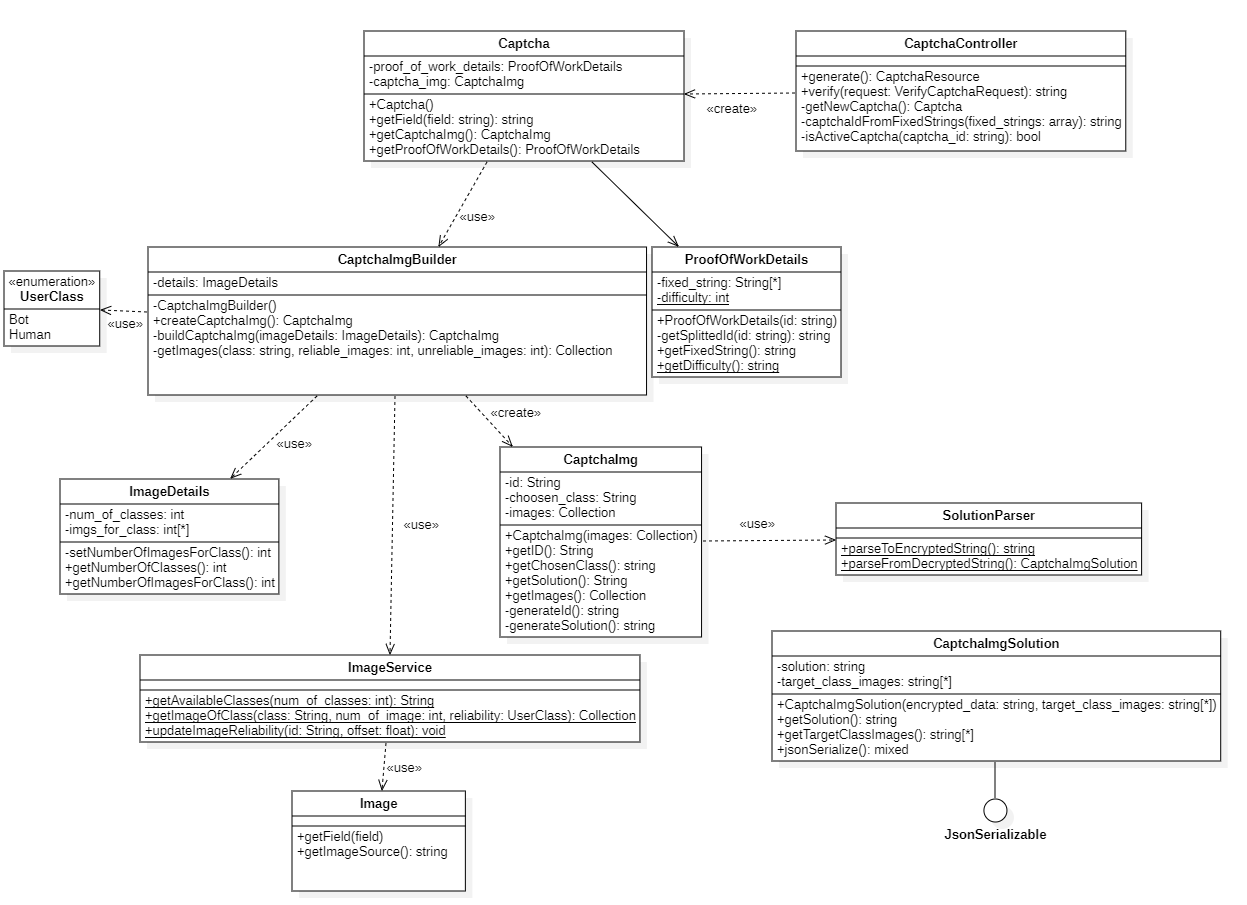
\includegraphics[scale = 0.45]{img/generate.png}\\
    \caption{Diagramma delle classi. Generazione del CAPTCHA\textsubscript{G}}
\end{figure}
\newpage

Nella figura sopra viene mostrata la logica utilizzata per la generazione di un  CAPTCHA\textsubscript{G}.
Ogni CAPTCHA\textsubscript{G} è composto da:
 \begin{itemize}
     \item 9 immagini in bianco e nero con solo i contorni visibili;
     \item L'immagine honeypot\textsubscript{G}, invisibile all'utente;
     \item Il Proof of work\textsubscript{G}.
 \end{itemize}


In particolare:
\begin{itemize}
    \item \textbf{CaptchaController}: Classe cardine del progetto, la quale si occupa di gestire tutte le richieste che verranno fatte all'API\textsubscript{G}. In questa classe è anche contenuto il metodo che ritornerà l'oggetto \textit{Resource} a seguito di una richiesta da parte dell'utente;
    \item \textbf{CAPTCHA\textsubscript{G}}: Classe che si occupa di mettere insieme tutti i pezzi che compongono il CAPTCHA\textsubscript{G}, ovvero immagini, honeypot\textsubscript{G} e proof of work\textsubscript{G}. Questa classe viene creata dal Controller quando viene richiesto un CAPTCHA\textsubscript{G};
    \item \textbf{CaptchaImgBuilder}: Classe che utilizza il pattern dependency injection e si occupa dell'effettiva creazione della parte del CAPTCHA\textsubscript{G} che contiene le immagini e l'honeypot\textsubscript{G}. Fa inoltre utilizzo di una enumerazione per la gestione dell'affidabilità delle immagini;
    \item \textbf{ProofOfWorkDetails}: Classe che contiene i dati necessari per il calcolo dei nonce nel proof of work\textsubscript{G};
    \item \textbf{ImageDetails}: Classe che contiene i dettagli utili alla creazione delle 9 immagini che comporranno il Captcha\textsubscript{G}, quali il numero di classi e di immagini per classe che dovrà avere. Viene utilizzata dalla classe \textit{CaptchaImgBuilder};
    \item \textbf{CaptchaImg}: Classe che contiene le varie informazioni che la parte del CAPTCHA\textsubscript{G} composta dalle immagini deve avere. È l'oggetto che la classe \textit{CaptchaImgBuilder} va a creare;
    \item \textbf{ImageService}: Classe che si interfaccia il DB al fine di recuperare informazioni e immagini necessarie alla creazione del CAPTCHA\textsubscript{G}. Viene utilizzata dalla classe \textit{CaptchaImgBuilder};
    \item \textbf{Image}: Eloquent Model che contiene le informazioni dell'oggetto immagine. Viene utilizzato da \textit{ImageService};
    \item \textbf{CaptchaImgSolution}: Classe che contiene le informazioni della soluzione della parte del CAPTCHA\textsubscript{G} composta dalle immagini;
    \item \textbf{Solution Parser}: Classe che fornisce i metodi per criptare e decriptare istanze della classe \textit{CaptchaImgSolution}.
\end{itemize}

\subsubsubsection{Captcha Resource}
\begin{figure}[H]
	\centering
	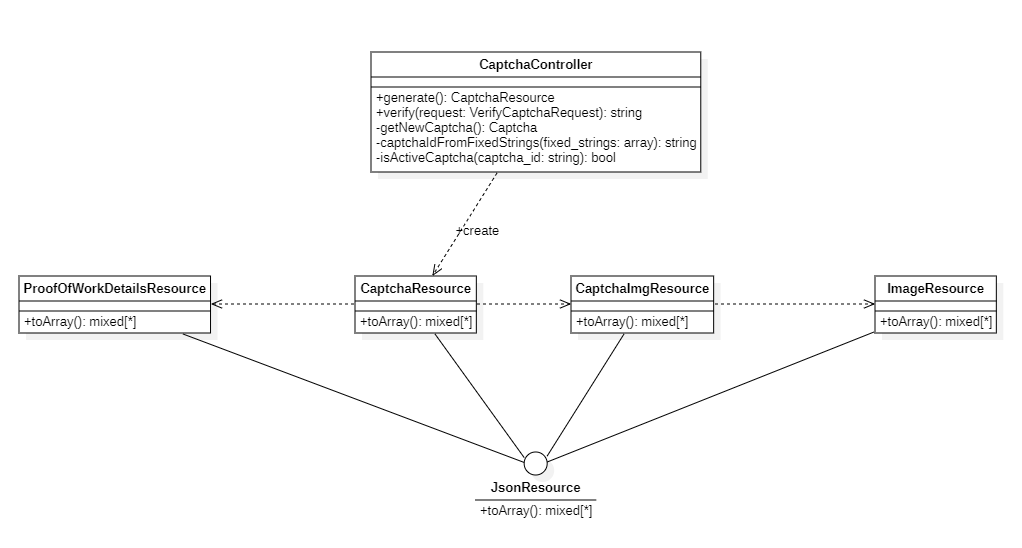
\includegraphics[scale = 0.6]{img/captcha_resource.png}\\
	\caption{Diagramma delle classi. Captcha resource}
\end{figure}

Nella figura sopra viene mostrata la logica utilizzata per la gestione delle informazioni che si vogliono passare all'utente al seguito di una richiesta. Infatti dopo la creazione di un CAPTCHA\textsubscript{G}, viene creato dal Controller l'oggetto \textit{CaptchaResource}, il quale sarà un JSON che contiene solamente le informazioni chiave per il caricamento del CAPTCHA\textsubscript{G} lato front-end e la soluzione criptata che servirà durante la verifica\textsubscript{G} del Captcha\textsubscript{G}. Le classi Resource, come suggerito dal framework\textsubscript{G} Laravel, vengono utilizzate per tradurre un Eloquent Model in formato JSON.

In particolare:
\begin{itemize}
	\item \textbf{CaptchaController}: Dopo aver creato il CAPTCHA\textsubscript{G}, genera l'oggetto \textit{CaptchaResource} il quale contiene le varie informazioni da passare in risposta alla richiesta dell'utente;
	\item \textbf{CaptchaResource}: Classe Eloquent Resource che utilizza le classi \textit{CaptchaImgResource} e \textit{ProofOfWorkDetailsResource} per generare il JSON che verrà poi inviato all'utente;
	\item \textbf{CaptchaImgResource}: Classe Eloquent Resource che seleziona le informazioni da inviare all'utente per la parte del CAPTCHA\textsubscript{G} immagini. Utilizza la classe \textit{ImageResource} per le informazioni delle immagini contenute nel Captcha\textsubscript{G};
	\item \textbf{ProofOfWorkDetailsResource}: Classe Eloquent Resource che seleziona le informazioni da inviare all'utente per la parte del proof of work\textsubscript{G};
	\item \textbf{ImageResource}: Classe Eloquent Resource che seleziona le informazioni che ogni immagine dovrà avere nella risposta all'utente.
\end{itemize}
\newpage

\subsubsubsection{Verifica\textsubscript{G} del CAPTCHA\textsubscript{G}}

\begin{figure}[H]
	\centering
	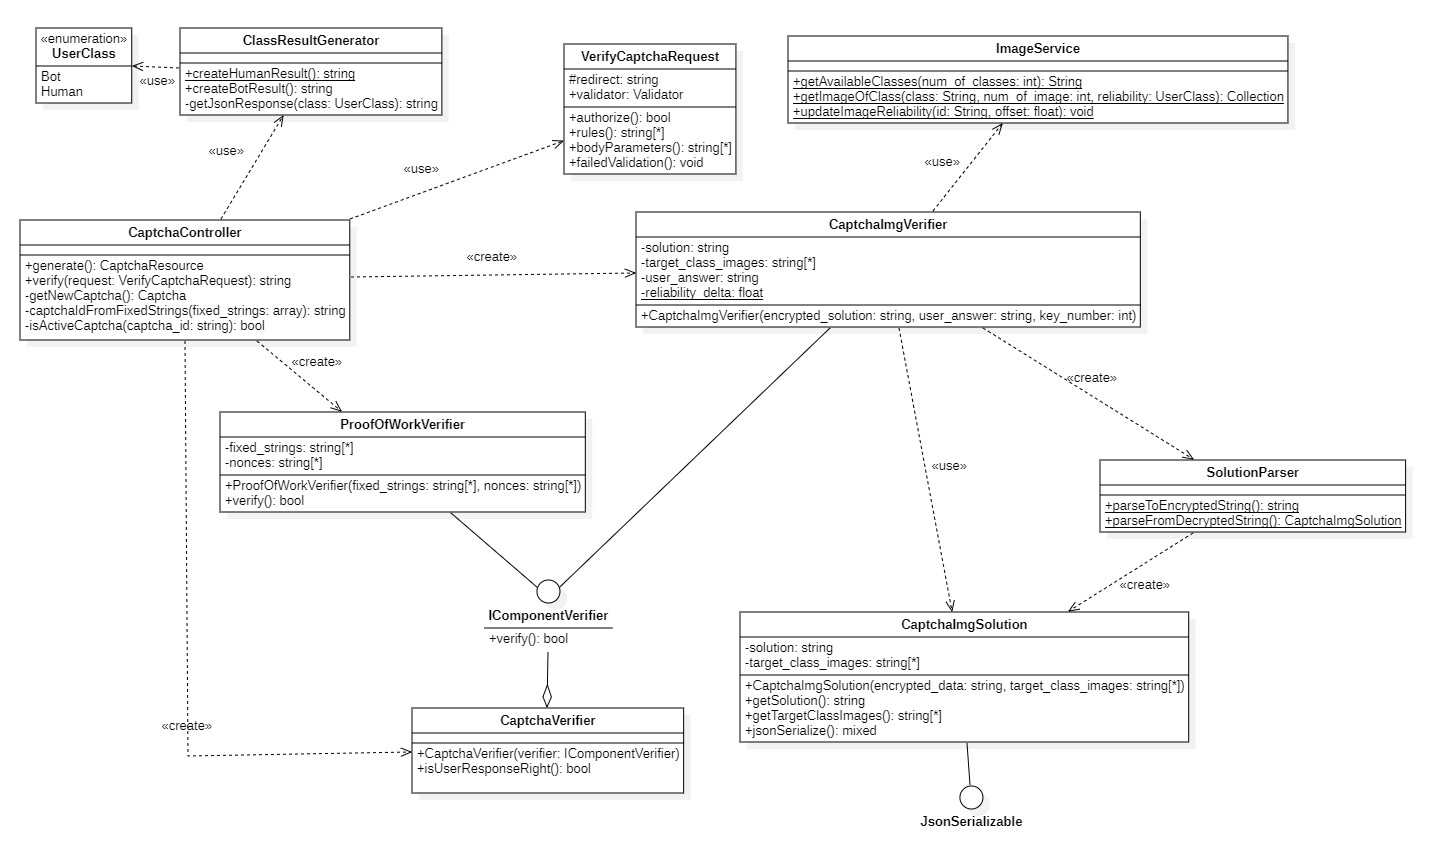
\includegraphics[scale = 0.45]{img/verify.png}\\
	\caption{Diagramma delle classi. Verifica\textsubscript{G} del CAPTCHA\textsubscript{G}}
\end{figure}

Nella figura sopra viene mostrata la logica utilizzata per la verifica\textsubscript{G} dei CAPTCHA\textsubscript{G} inviati dagli utenti. \textit{CaptchaController} riceve la richiesta e inizializza il verificatore passandogli i rispettivi verificatori del CAPTCHA\textsubscript{G} immagini e del proof of work\textsubscript{G}.
In particolare:
\begin{itemize}
	\item \textbf{VerifyCaptchaRequest}: Dopo aver ricevuto la richiesta, Laravel costruisce un oggetto di questa classe la quale estende la classe astratta \textit{Request}, verificando che sia conforme al set di regole specificato. Nel caso in cui il controllo fallisca, viene restituito un messaggio di errore con status code 400;
	\item \textbf{CaptchaController}: Questa classe si occupa di gestire le richieste per la verifica\textsubscript{G} di un CAPTCHA\textsubscript{G} andando a creare i verificatori che andranno a controllare la correttezza effettiva del CAPTCHA\textsubscript{G};
	\item \textbf{CaptchaVerifier}: Questa classe utilizza dei \textit{ComponentVerifier} per controllare se la risposta dell'utente è corretta o meno;
	\item \textbf{IComponentVerifier}: Questa interfaccia possiede il metodo verify che verrà implementato dai due verificatori;
	\item \textbf{CaptchaImgVerifier}: Classe che \textsubscript{G} la correttezza della soluzione dell'utente per la parte del CAPTCHA\textsubscript{G} composto dalle immagini, andando inoltre ad utilizzare la classe \textit{ImageService} per aggiornare l'affidabilità delle immagini nel DB;
	\item \textbf{ProofOfWorkVerifier}: Classe che verifica la correttezza dei nonce calcolati dall'utente durante il proof of work\textsubscript{G};
	\item \textbf{SolutionParser}: Classe utilizzata da \textit{CaptchaImgVerifier} per decriptare e costruire un'istanza della classe \textit{CaptchaImgSolution};
	\item \textbf{CaptchaImgSolution}: Classe che contiene gli attributi della soluzione del CAPTCHA\textsubscript{G}. Creata da \textit{SolutionParser} per fornire la soluzione decriptata a \textit{CaptchaImgVerifier};
	\item \textbf{ImageService}: Classe utilizzata dal \textit{CaptchaImgVerifier} per aggiornare l'affidabilità delle immagini della classe target all'interno del DB;
	\item \textbf{ClassResultGenerator}: Classe che codifica il risultato criptandolo utilizzando una chiave simmetrica.
\end{itemize}

\newpage

\subsubsubsection{Gestione delle chiavi e dell'encrypting}

\begin{figure}[H]
	\centering
	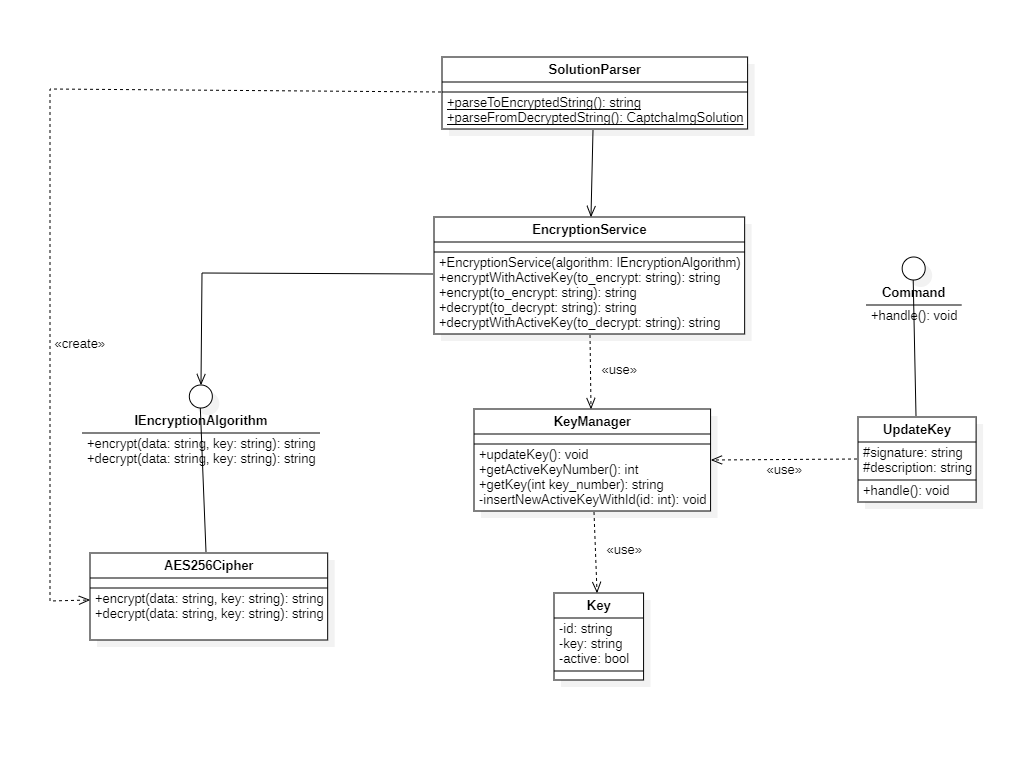
\includegraphics[scale = 0.55]{img/key_manager.png}\\
	\caption{Diagramma delle classi. Gestione delle chiavi e dell'encrypting}
\end{figure}

Nella figura sopra viene mostrata la logica utilizzata per la gestione delle chiavi con cui vengono criptate le soluzioni dei CAPTCHA\textsubscript{G} creati, ma anche la struttura in cui alla base c'è l'algoritmo\textsubscript{G} che cripta e decripta le soluzioni.\\
In particolare:
\begin{itemize}
	\item \textbf{SolutionParser}: Questa classe si occupa di criptare e decriptare le soluzioni dei CAPTCHA\textsubscript{G} utilizzando la classe \textit{EncryptionService};
	\item \textbf{EncryptionService}: Classe che implementa i metodi crypt e decrypt per le diverse situazioni in cui sono richiesti;
	\item \textbf{IEncryptionAlgorithm}: Questa interfaccia possiede i metodi crypt e decrypt che verranno implementati dalla classe \textit{AES256Cipher};
	\item \textbf{AES256Cipher}: Classe che implementa i metodi crypt e decrypt attraverso la chiave fornita e l'algoritmo\textsubscript{G} AES256;
	\item \textbf{KeyManager}: Classe che contiene i vari metodi che permettono di inserire, recuperare e aggiornare le chiavi nel DB;
	\item \textbf{Key}: Eloquent Model che contiene i vari attributi che una chiave deve possedere. Utilizzato dalla classe \textit{KeyManager};
	\item \textbf{UpdateKey}: Derivata dalla classe Command di Laravel. Gestisce la chiamata del metodo per l'aggiornamento di una chiave nel DB presente in \textit{KeyManager}. Questo comando è eseguito ogni minuto dallo scheduler definito dal framework\textsubscript{G}.
\end{itemize}

\newpage

\subsubsubsection{Download e elaborazione delle immagini}

\begin{figure}[H]
    \centering
    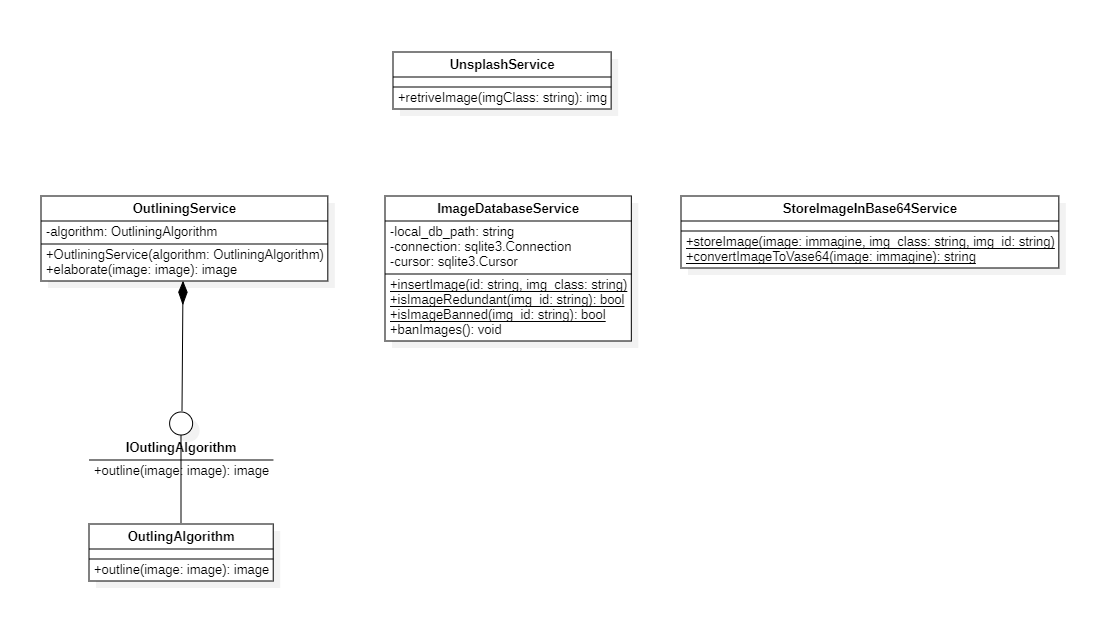
\includegraphics[scale = 0.6]{img/downloadImg.png}\\
    \caption{Diagramma delle classi. Recupero delle immagini da Unsplash}
\end{figure}

La figura sopra riportata rappresenta le varie classi e interfacce che sono utilizzate dallo script\textsubscript{G} per il download delle immagini dal sito di Unsplash, la rielaborazione di tali immagini e il salvataggio di esse.\\ Questo processo segue il seguente ordine:
\begin{enumerate}
	\item Inizialmente viene fatto un controllo per vedere se ci sono immagini con un'affidabilità troppo bassa e quindi eliminarle dal DB;
    \item Dopodiché viene scaricata una nuova immagine di una determina classe da Unsplash;
    \item Viene compiuta l'elaborazione dell'immagine eliminando i colori e tenendo solo il contorno;
    \item Viene quindi convertita in base64\textsubscript{G};
    \item Infine l'immagine viene salvata e inserita nel DB.
\end{enumerate}
\newpage
In particolare:
\begin{itemize}
    \item \textbf{UnsplashService}: Classe che si occupa di fare la richiesta di un immagine al servizio di Unsplash;
    \item \textbf{OutliningService}: Classe che si occupa dell'elaborazione dell'immagine;
    \item \textbf{IOutliningAlgorithm}: Interfaccia che contiene il metodo che sarà poi implementato nella classe \textit{OutilningAlgorithm} per l'elaborazione delle immagini;
    \item \textbf{OutilningAlgorithm}: Classe che implementa l'algoritmo\textsubscript{G} di elaborazione dell'immagine;
    \item \textbf{StoreImageInBase64Service}: Classe si occupa della conversione in base64\textsubscript{G} dell'immagine e del suo salvataggio usando come path \textit{classe/id\_immagine};
    \item \textbf{ImageDatabaseService}: Classe che implementa i vari metodi per eliminare, inserire e fare controlli sulle immagini nel DB.
\end{itemize}
\newpage
\subsubsection{Front-end}
La parte del front-end del progetto, è completamente separata dall'API\textsubscript{G} che offre il servizio CAPTCHA\textsubscript{G} ed è composta da:
\begin{itemize}
	\item Pagina di login, nella quale l'utente può richiedere un CAPTCHA\textsubscript{G}, 
    compilarlo e fare di conseguenza l'accesso;
    \item Un file JS che si occupa del calcolo del proof of work\textsubscript{G};
    \item Un file JS che si occupa di inserire dinamicamente i dati ricevuti in risposta dal servizio nella pagina e di far iniziare il proof of work\textsubscript{G}.
\end{itemize}
Il lato client, per poter fare le richieste al servizio, fa utilizzo anch'esso di una classe Controller, la quale possiede due metodi che vengono chiamati nel caso l'utente voglia generare un CAPTCHA\textsubscript{G} o di verificarne uno. Questi metodi si occupano di fare le richieste effettive all'API\textsubscript{G}, ottenendo i dati in risposta che saranno poi gestiti tramite JS, nel caso della generazione o nel caso della verifica\textsubscript{G} di reindirizzare l'utente in base alla correttezza o meno della risposta inviata.
Anche questa classe è completamente sconnessa dall'API\textsubscript{G} e si occupa solo di fare le richieste la servizio. 

\begin{figure}[H]
	\centering
	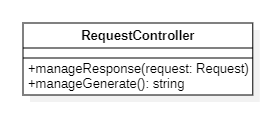
\includegraphics[scale = 0.8]{img/request_controller.png}\\
	\caption{Controller per le richieste dell'utente}
\end{figure}

\subsection{Architettura\textsubscript{G} di dettaglio}

\subsubsection{Strategy pattern}

\begin{figure}[H]
    \centering
    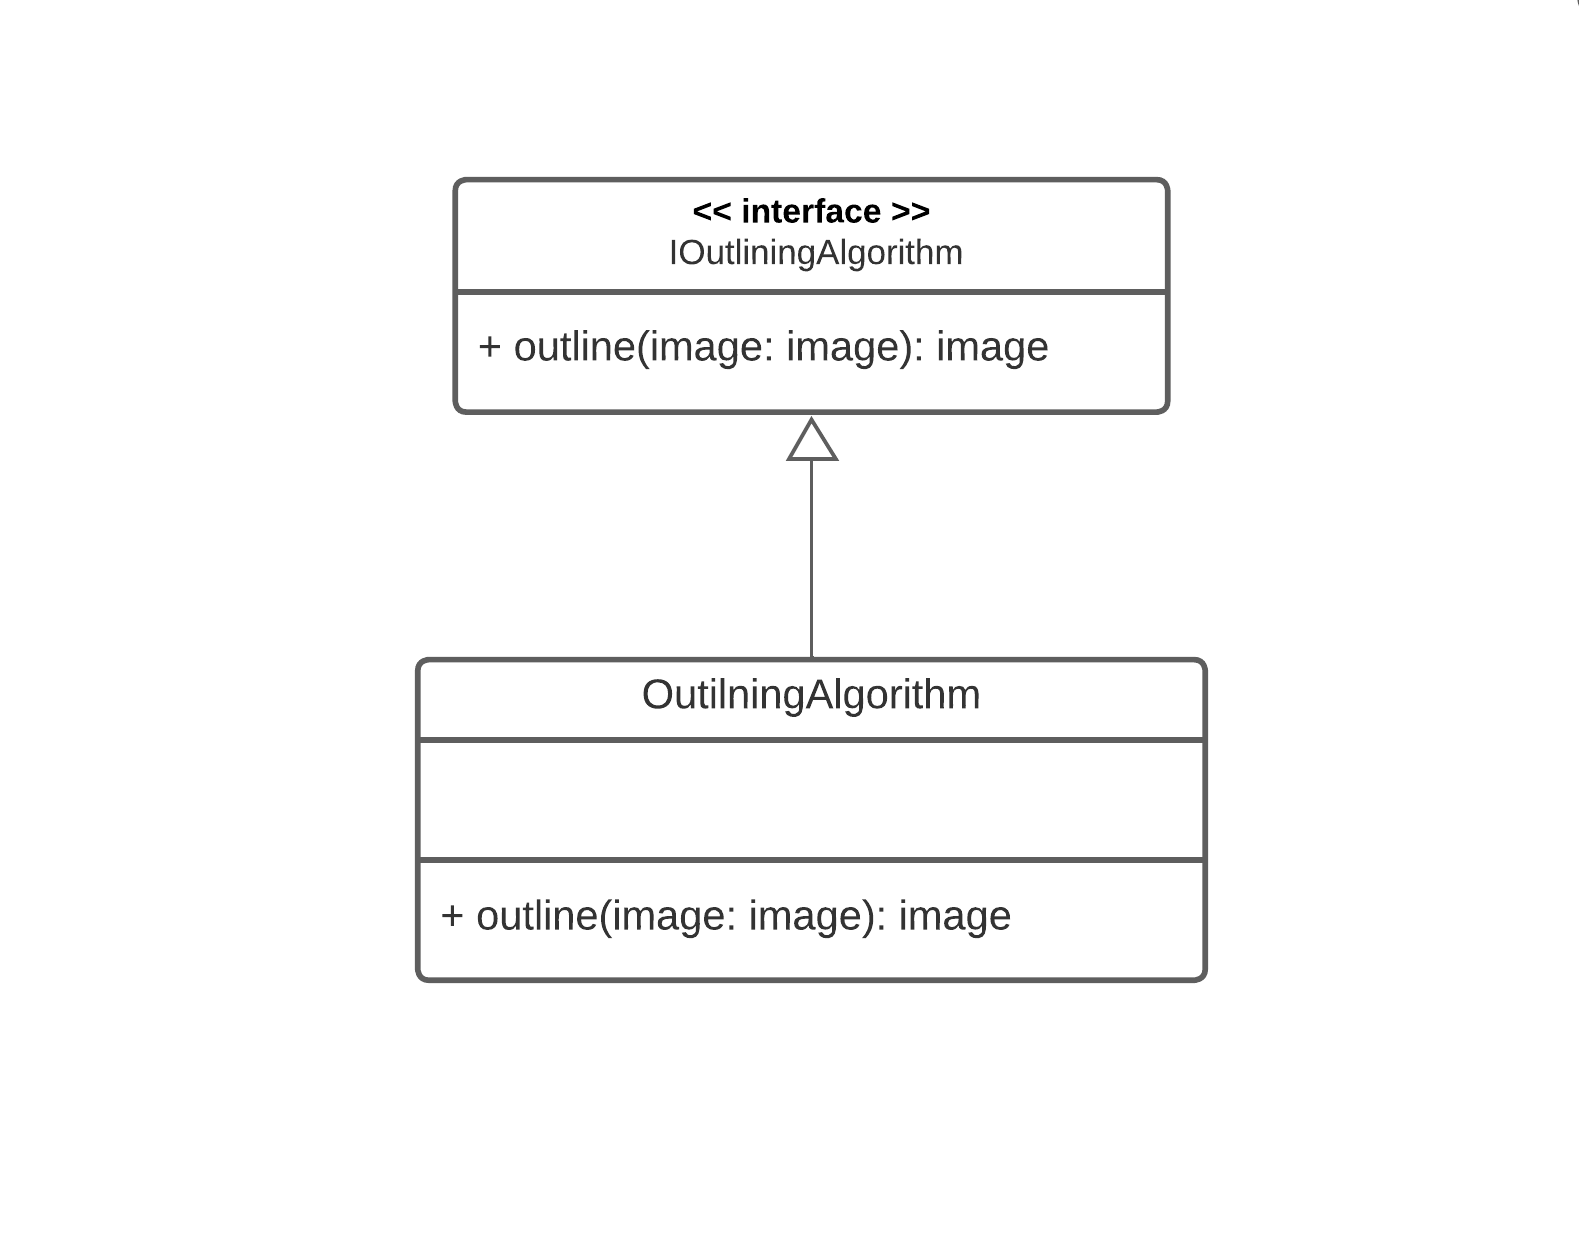
\includegraphics[scale = 0.8]{img/outlineStrategy.png}\\
    \caption{Strategy pattern dell'algoritmo\textsubscript{G} di rielaborazione dell'immagine}
\end{figure}

Attualmente, l'interfaccia \textit{IOutliningAlgorithm} ha una sola classe concreta che rappresenta l'unico algoritmo\textsubscript{G} implementato. Tuttavia, è progettata in modo da consentire l'estensione per l'implementazione di ulteriori 
algoritmi in futuro. Ciò significa che se si desidera aggiungere nuovi algoritmi di scontorno delle immagini sarà possibile farlo creando nuove classi che estendono l'interfaccia \textit{IOutliningAlgorithm}. 
Questa flessibilità consente di espandere il sistema per includere più algoritmi di scontorno delle immagini senza dover 
modificare la struttura di base.

\begin{figure}[H]
    \centering
    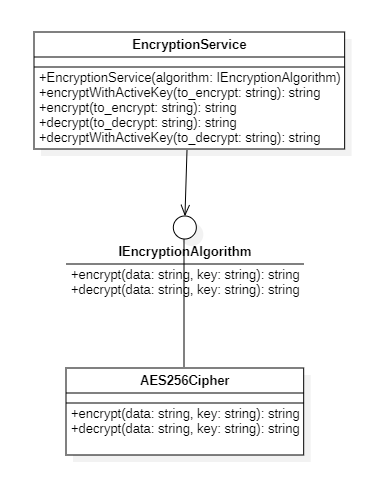
\includegraphics[scale = 0.8]{img/cryptStrategy.png}\\
    \caption{Strategy patter dell'algoritmo\textsubscript{G} per l'encrypting}
\end{figure}

L'interfaccia \textit{IEncryptionAlgorithm} possiede una sola classe concreta per lo stesso motivo citato precedentemente. In questa maniera, l'implementazione di un nuovo algoritmo\textsubscript{G} di crittografia risulterà semplice e non richiederà la modifica di codice esistente.

\subsubsection{Dependency Injection}

\begin{figure}[H]
    \centering
    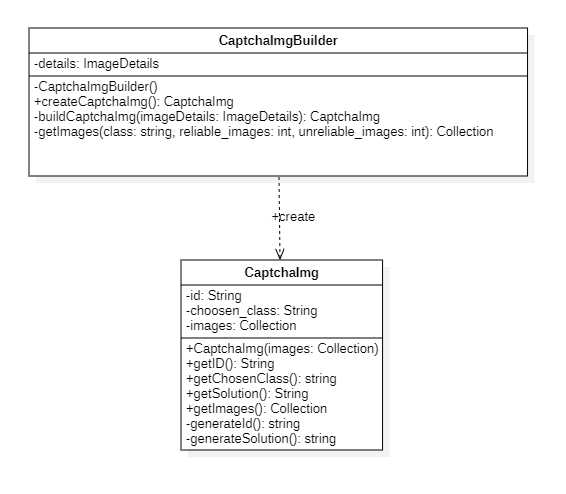
\includegraphics[scale = 0.7]{img/dependency_injection.png}\\
    \caption{Dependency injection pattern}
\end{figure}

La costruzione di un'istanza di \textit{CaptchaImg} è un'operazione che può essere considerata complessa in quanto bisogna tenere in considerazione diverse variabili, ad esempio il numero di classi di immagine presenti e numero di immagini per classe. \\
Tutte queste variabili sono contenute all'interno della classe \textit{ImageDetails} dove vengono definite le condizioni per ognuna di esse:
\begin{itemize}
    \item Numero di classi tra 2 e 4 estremi compresi;
    \item 9 immagini totali;
    \item Le immagini della classe target devono essere la metà + 1 affidabili;
    \item Le immagini delle classi non target devono essere la metà affidabili.
\end{itemize}
Per quanto elencato sopra si è deciso quindi di spezzare la complessità e creare una classe il cui compito è quello di rifornire il costruttore di \textit{CaptchaImg}. 